\chapter{Classical Visual State Estimation}

\section{Visual Odometry Pipeline}

The learned pseudo-sensors in this thesis are applied to a standard visual odometry pipeline largely based on the work of \cite{furgale_phd11}. We briefly summarize the pipeline here, and outline any unique design choices we made.


\begin{figure}
\begin{center}
		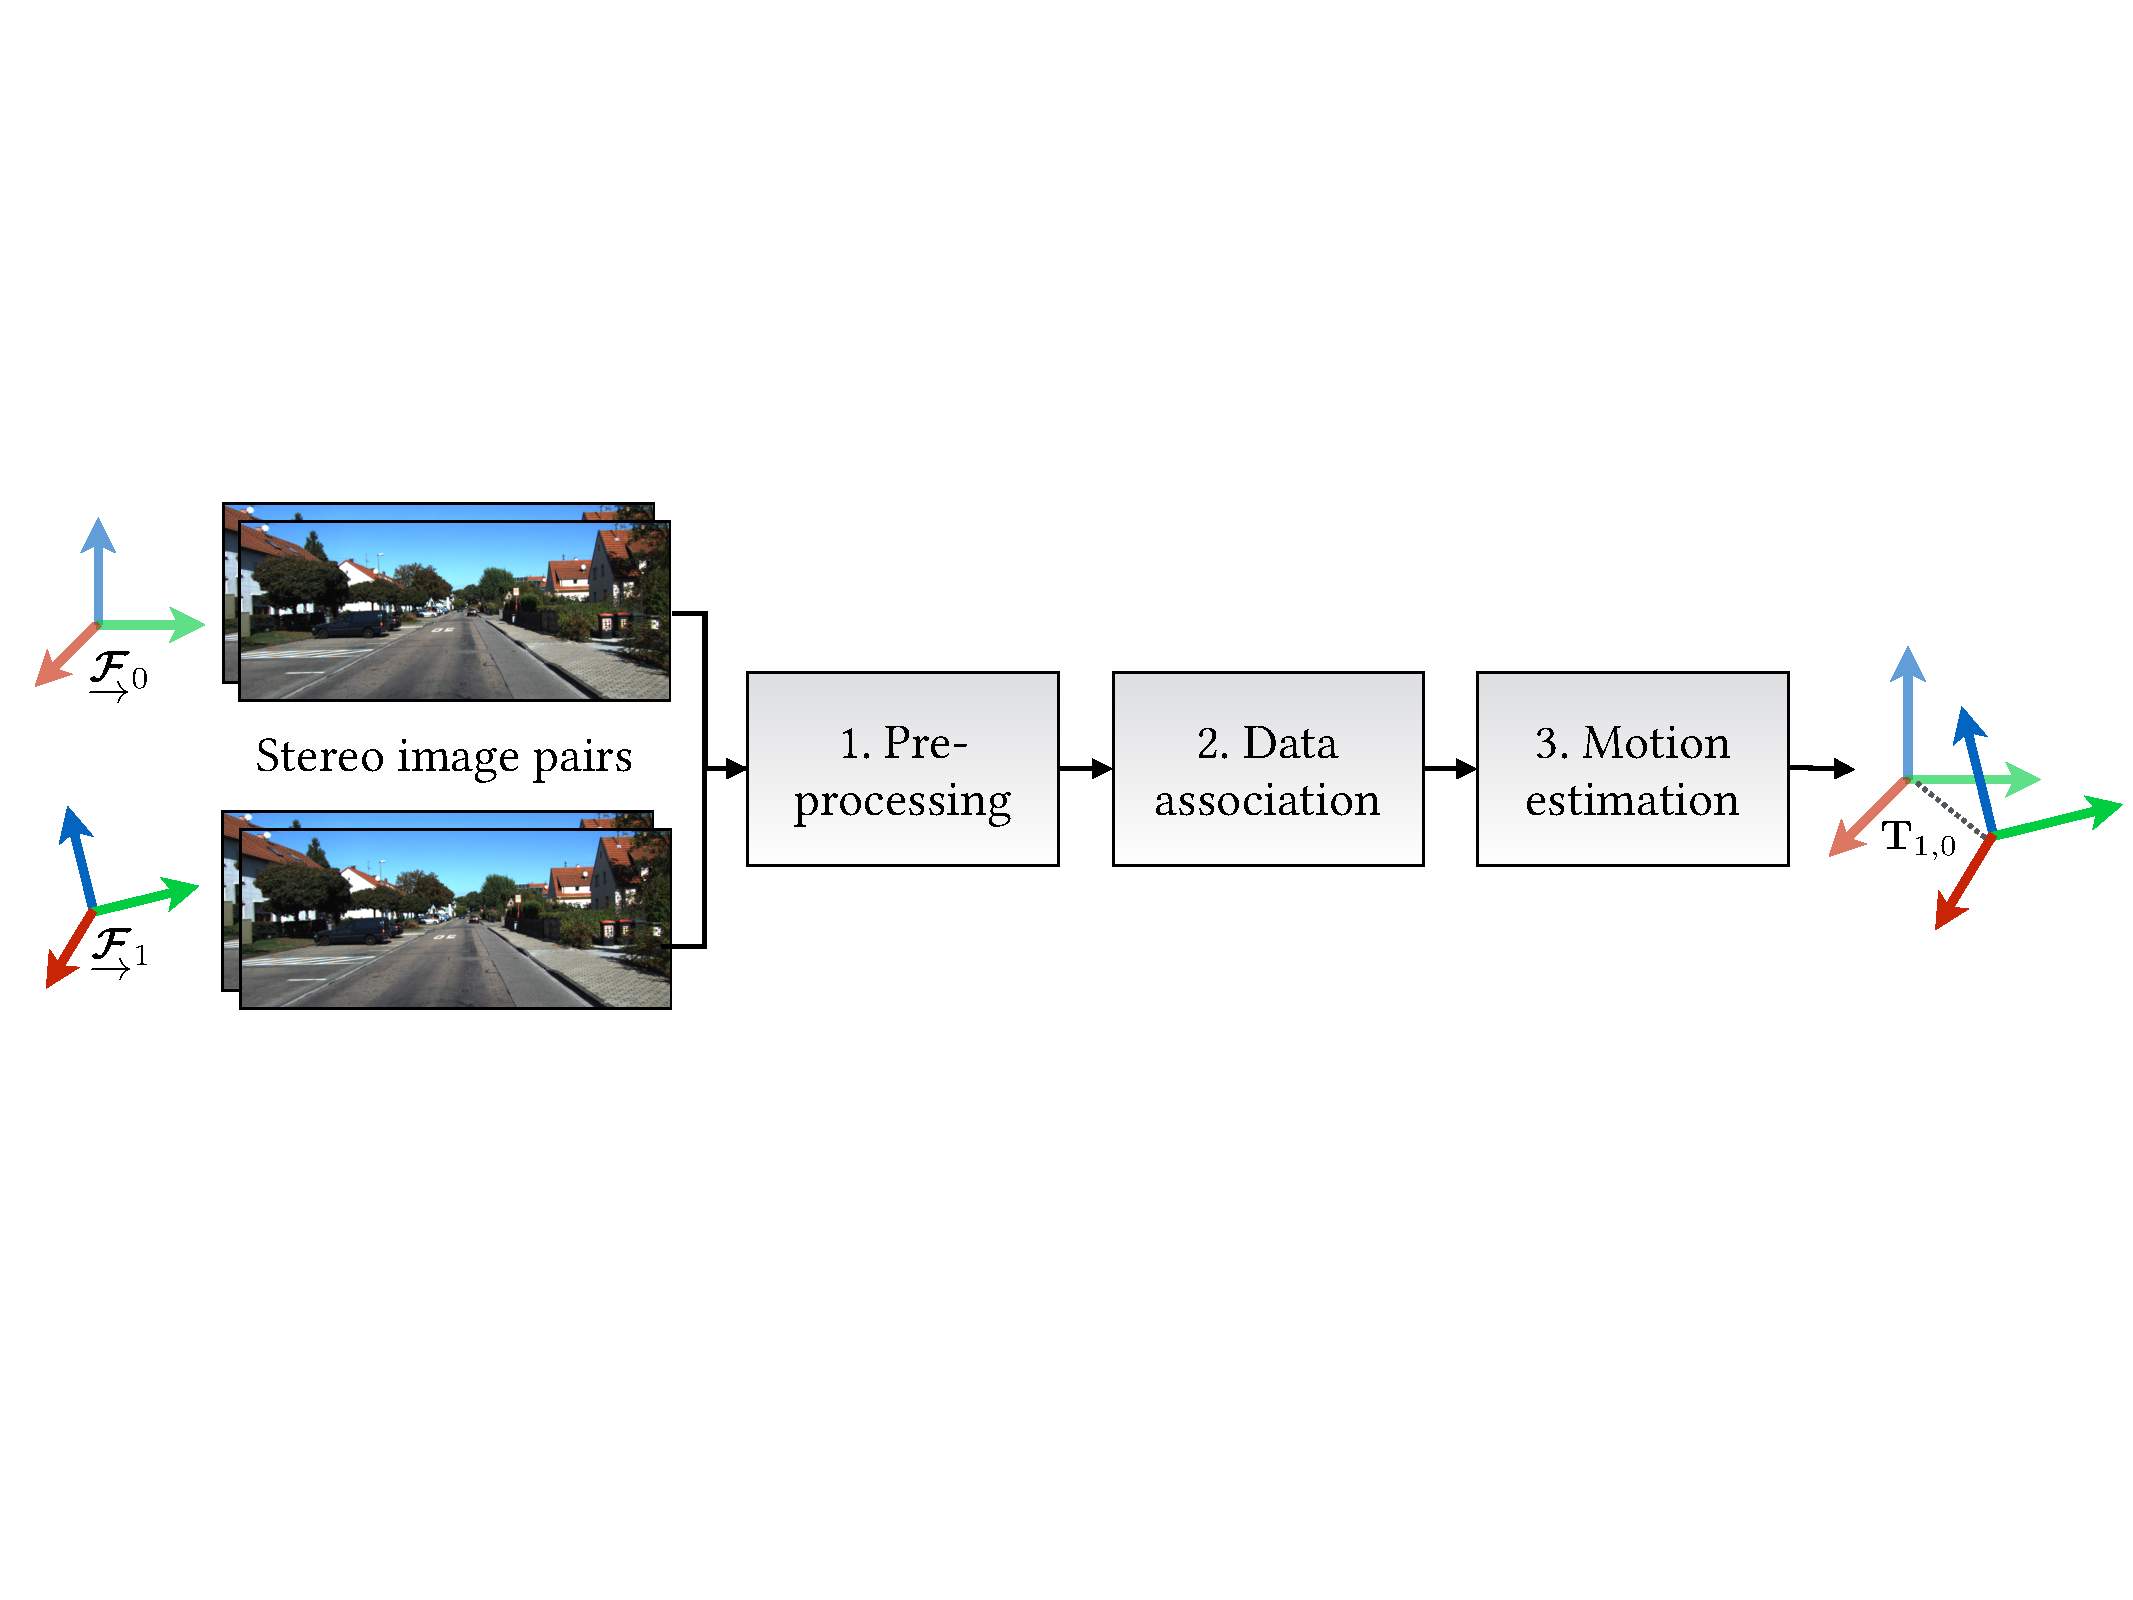
\includegraphics[width=0.98\textwidth]{math/stereo_vo_pipeline.pdf}
		\caption{A `classical' stereo visual odometry pipeline consists of several distinct components that have interpretable inputs and outputs.}
  	\label{fig:math_stereo_vo_pipeline}
\end{center}
\end{figure}

\subsection{Pre processing}

\begin{figure}
\begin{center}
		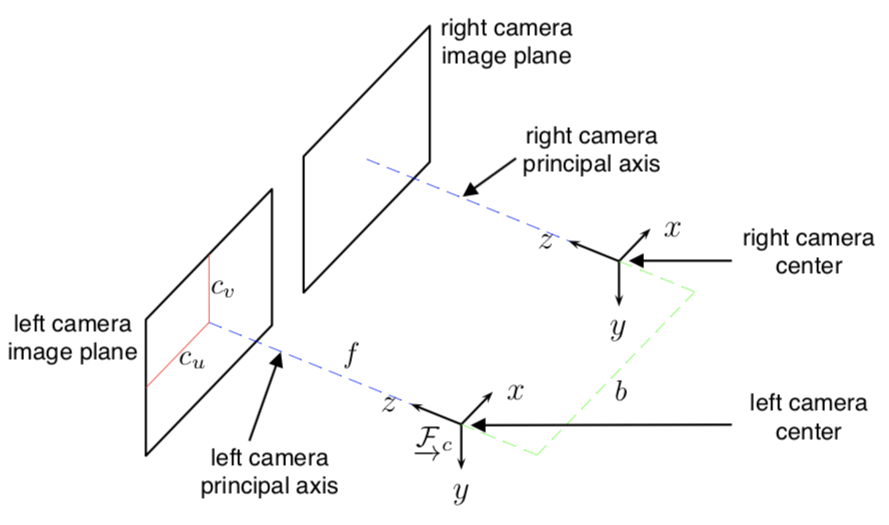
\includegraphics[width=0.98\textwidth]{math/stereo_camera_rectified}
		%\tdplotsetmaincoords{-60}{-35}
\begin{tikzpicture}
  [
    tdplot_main_coords,
    >=Stealth,
    my dashed/.style={dashed, thick, ->, shorten >=-15pt, shorten <=-15pt, every node/.append style={font=\footnotesize}},
    my box/.style={thin, gray!70},
    my blue/.style={blue, line cap=round, -{Triangle[width=3*#1]}, line width=#1, shorten >=#1*1.75pt, every node/.append style={fill, circle, inner sep=0pt, minimum size=#1*3.5pt, anchor=center, outer sep=0pt}},
    my label/.append style={midway, font=\scriptsize},
    my vectors/.style={green!50!black, {Stealth[scale=.75]}-{Stealth[scale=.75]}},
    my red/.style={thick, red, line cap=round},
    my grey/.style={gray!70},
    description/.style={draw=gray!70, thick, line cap=round, every node/.style={align=center, font=\scriptsize\sffamily, anchor=north}},
  ]
%   \draw [help lines] (-2,0,0) -- (2,0,0) node[anchor=north west]{$x$} (0,0,0) -- (0,7,0) node[anchor=north east]{$y$} (0,0,0) -- (0,0,2) node[anchor=north]{$z$} (-2,7,0) -- (2,7,0);
  \draw [my grey] (0,4,0) -- (0,7,0) (-2,7,0) -- (2,7,0);
  \coordinate (o) at (0,0,0);
  \path [draw=gray!70, text=gray, fill=gray!20, opacity=0.8, text opacity=1] (-1.5,4,1.75) coordinate (a) -- ++(0,0,-3.5) coordinate (b) -- ++(3,0,0) coordinate (c) -- ++(0,0,3.5) coordinate (d) -- cycle node [pos=.95, above, sloped, anchor=south west] {$z=f$} ;
%   \foreach \i in {a,b,c,d} \node [red, font=\scriptsize] at (\i) {\i};
  \draw [my grey] (-2,0,0) -- (2,0,0) (0,0,0) -- (0,4,0) (0,0,0) -- (0,0,2);
  \draw [thick, ->, every node/.style={font=\footnotesize, inner sep=0pt}] (o) node [anchor=north west] {$F_c$} (o) edge node [pos=1, anchor=north east] {$z_c$} ++(0,1,0) edge node [pos=1, anchor=north] {$y_c$} ++(0,0,1) -- ++(1,0,0) node [anchor=north west] {$x_c$};
  \draw [my box] (o) ++(0,4,-.5) coordinate (p1) -- ++(1,0,0) coordinate (p2) -- ++(0,0,-1.25) coordinate (p3);
  \foreach \i in {0,1,...,4} \draw [my box] (p1) ++(\i*.25,0,0) -- ++(0,0,-.25);
  \foreach \i in {0,1,...,5} \draw [my box] (p2) ++(0,0,-\i*.25) -- ++(-.25,0,0);
  \draw [my box] (p1) ++(0,0,-.25) -- ++(.75,0,0) -- ++(0,0,-1);
  \draw [my dashed, cyan] ($(b)!1/2!(c)$) -- ($(d)!1/2!(a)$) node [below=15pt, anchor=north] {$y$};
  \draw [my dashed, cyan] ($(b)!1/2!(a)$) -- ($(d)!1/2!(c)$) node [above right=17pt, anchor=north west] {$x$};
  \draw [my dashed, green!50!black, <->] (a) node [below=15pt, anchor=north] {$v$} -- (b) -- (c) node [above right=17pt, anchor=north west] {$u$};
  \path [green!50!black, every node/.style={font=\scriptsize, inner sep=0pt}] (p2) node [above right, anchor=south west] {$(u,v)$};
  \path (p2) ++(-.125,0,0) coordinate (q2) ++(0,0,-.125) coordinate (r2);
  \draw [my blue=1] ($(0,4,0)+($(q2)-(p1)$)$) coordinate (s2) -- (r2) node (d1) {};
  \scoped[on background layer]{\draw [my blue=1.75] ($($1.75*($(s2)-(0,4,0)$)$)+(0,7,0)$) -- ++($1.75*($(r2)-(s2)$)$) node (d2) [label={[label distance=-20pt]above:{$P=(X,Y,Z)$}}] {};}
  \draw [my vectors] (0,4,.1) -- ($(s2)+(0,0,.1)$) node [below, my label, sloped] {$\vec{u}$};
  \draw [my vectors] (-.1,4,0) -- ($(q2)-(s2)+(-.1,4,0)$) node [left, my label] {$\vec{v}$};
  \draw [my red] (o) -- (d1.center);
  \scoped[on background layer]{\draw [my red] (d1.center) -- (d2.center);}
  \path [description] (0,4,0) [out=-95, in=95] to (-.75,4,.25) node {principal\\point} (0,6.5,0) [out=-95, in=95] to (-.75,6.5,.25) node {optical\\axis};
\end{tikzpicture}

		\caption{A rectified stereo camera with equal focal lengths. Taken \cite{furgale_phd11}. \todo{reproduce myself}.}
  	\label{fig:math_stereo_camera}
\end{center}
\end{figure}

In the preprocessing stage, stereo images are undistorted and rectified such that their principal axes are parallel, see \Cref{fig:math_stereo_camera}. We assume the stereo camera intrinsic and extrinsic parameters as well as the lens properties are known a priori (or computed through a calibration process like that detailed in \cite{kelly_phd2011}).

\subsection{Data association}

\subsubsection{Feature extraction and matching}

During data association, some form of image features must be matched. In this thesis, we focus on sparse stereo visual odometry which uses the \texttt{libviso2} image feature extraction and matching mechanism.  

Each landmark corresponds to a
point in space, expressed in homogeneous coordinates in the camera frame as
$\HomogeneousPoint{i}{t} := \Transpose{\bbm p_1 & p_2 & p_3 & p_4 \ebm} \in
\HomogeneousNumbers[3]$.  The stereo-camera model, $\ProjectionFunction$,
projects a landmark expressed in homogeneous coordinates into image space, so
that $\ImageLandmark{i}{t}$, the stereo pixel coordinates of landmark $i$ in the first camera pose at time $t$, is given
by 
\begin{equation}
	\ImageLandmark{i}{t} = \bbm u_l \\ v_l \\ u_r \\ v_r \ebm 
  = \ProjectionFunction(\HomogeneousPoint{i}{t}) 
  = \Matrix{M} \frac{1}{p_3}\HomogeneousPoint{i}{t},
\end{equation}
where
\begin{equation}
 \Matrix{M} = \bbm f_u & 0 & c_u & f_u \frac{b}{2} \\ 0 & f_v & c_v & 0 \\ f_u 
                        & 0 & c_u & -f_u\frac{b}{2} \\ 0 & f_b & c_v & 0 \ebm.
\end{equation}
Here, $\{c_u, c_v\}$, $\{f_u, f_v\}$, and $b$ are the principal points, focal
lengths and baseline of the stereo camera respectively. Note that in this
formulation, the stereo camera frame is centered between the two individual
lenses.  


\subsubsection{Outlier rejection}

Brief description of RANSAC and Horn's method.

\subsection{Motion solution}

In our frame-to-frame sparse stereo odometry pipeline,  the objective is to find
$\Transform_t\in\text{SE}(3)$, the rigid transform between two subsequent stereo camera poses (note that the temporal index $t$ refers to the set of two stereo camera poses). We begin by rectifying, then stereo and temporally
matching the set of 4 images to generate the corresponding locations of a set
of $N_t$ visual landmarks in each stereo pair.  

We triangulate landmarks in the first camera frame, $\ImageLandmark{i}{t}$, and re-project
them into the second frame, $\ImageLandmark{i}{t}'$. We model errors due to sensor noise
and quantization as a Gaussian distribution in image space with a known covariance
$\Covariance$,
\begin{equation}
  p(\ImageLandmark{i}{t}' \vert \ImageLandmark{i}{t}, \Transform_t,
  \Covariance)
  =\NormalDistribution\left(\Vector{e}_{i,t}(\Transform_t); \Vector 0, \Covariance\right), 
\end{equation}
where
\begin{equation}
 \Vector{e}_{i,t} = \ImageLandmark{i}{t}' - \ProjectionFunction( \Transform_t 
    \ProjectionFunction^{-1}( \ImageLandmark{i}{t} ) ).	
   \label{eq:image_error}
\end{equation}
  The maximum likelihood transform,
$\Transform_t^*$, is then given by 
\begin{equation}
  \Transform_t^* = \ArgMin{\Transform_t\in\text{SE}(3)}\sum_{i=1}^{N_t} 
  \Transpose{\Vector{e}_{i,t}} \Covariance^{-1} \Vector{e}_{i,t}.
\end{equation}
This is a nonlinear least squares problem, and can be solved iteratively using
standard techniques. During iteration $n$, we represent the transform as the
product of an estimate $\Transform^{(n)}\in\text{SE}(3)$ and a perturbation
$\delta\Vector{\xi}\in\RealNumbers[6]$ represented in exponential
coordinates:
\begin{equation}
  \Transform_t = \exp{\left( \delta\Vector{\xi}^{\wedge}
  \right)} \Transform_t^{(n)}.
\end{equation}
Linearizing the transform for small perturbations $\delta\Vector{\xi}$
yields a linear least-squares problem:
\begin{equation}
  \mathcal{L}(\delta \Vector{\xi}) = \frac{1}{2}\sum_{i=1}^{N_t} 
  \Transpose{\left(\Vector{e}_{i,t}^{(n)}
  - \Matrix J_{i,t}^{(n)} \delta\Vector{\xi}\right)}
\Covariance^{-1}
 \left(\Vector{e}_{i,t}^{(n)}
 - \Matrix J_{i,t}^{(n)} \delta\Vector{\xi}\right)
  \end{equation}
Here, $\Matrix J_{i,t}^{(n)}$ is the Jacobian matrix of the reprojection error.
The explicit form of the Jacobian matrix is omitted for brevity but can be
found in our supplemental materials.

Rearranging, we see the minimizing perturbation is the solution to a
linear system of equations:
\begin{equation}
  \delta\Vector{\xi}^{(n)} = 
  \left( \sum_{i=1}^{N_t} \Transpose{\Matrix J}_{i,t}
  \ImageLandmarkCovariance{}{}^{-1} \Matrix J_{i,t} \right)^{-1}
  \sum_{i=1}^{N_t} \Transpose{\Matrix J}_{i,t}
  \Covariance^{-1} \Vector{e}_{i,t}^{(n)}. 
\label{eq:least-squares-iteration}
\end{equation}
We then update the estimated transform and proceed to the next iteration.
\begin{equation}
  \Transform_t^{(n+1)} = \exp{\left( \delta\Vector{\xi}^{(n)\wedge}
  \right)} \Transform_t^{(n)}. \label{eq:update}
\end{equation}
There are many reasonable choices for both the initial transform
$\Transform_t^{(0)}$ and for the conditions under which we terminate
iteration. We initialize the estimated transform to identity, and iteratively
perform the update given by \cref{eq:update} until we see a relative change in
the squared error of less than one percent after an update. 


\section{Pose Graph Relaxation}

we fused our probabilistic rotation regression with classical stereo visual odometry using pose graph relaxation implemented with the help of a Python-based factor graph library which we will publicize after the review process. Using that framework, we solved
\begin{align}
	\Transform_{1,w}^*, \Transform_{2,w}^* &= \ArgMin{\Transform_{1,w}, \Transform_{2,w}\in\text{SE}(3)}\mathcal{L}(\Estimate{\Transform}_{2,1}, \Estimate{\Rotation}_{2,1}) \\ & = \ArgMin{\Transform_{1,w}, \Transform_{2,w}\in\text{SE}(3)} \Vector{\xi}_\text{1,2}^T \Matrix{\Sigma}^{-1}_\text{vo} \Vector{\xi}_\text{1,2} + \Vector{\phi}_\text{1,2}^T \Matrix{\Sigma}^{-1}_{\text{hn}} \Vector{\phi}_\text{1,2} 
\end{align}
where
\begin{equation}
	\Vector{\xi}_\text{1,2} =  \MatLog{\left(\Transform_{2,w} \Transform_{1,w}^{-1} \right)\Estimate{\Transform}_{2,1}^{-1}},
\end{equation}
\begin{equation}
	\Vector{\phi}_\text{1,2} =  \MatLog{\left(\Rotation_{2,w} \Rotation_{1,w}^{T} \right)\Estimate{\Rotation}_{2,1}^{T}},
\end{equation}
and $\Estimate{\Transform}_{2,1}$, $\Matrix{\Sigma}_\text{vo}$ and $\Estimate{\Rotation}_{2,1}$, $\Matrix{\Sigma}_{\text{hn}}$ were provided by our classical estimator and the HydraNet network respectively. Note that $\Matrix{\Sigma}_{\text{hn}} \in \Real^{3 \times 3} \geq 0$ while $\Matrix{\Sigma}_{\text{vo}} \in \Real^{6 \times 6} \geq 0 $. We also overload the logarithm function, $\MatLog{\cdot}$ to represent both $\LieGroupSE{3}$ and $\LieGroupSO{3}$ logarithmic maps as necessary. To account for gauge freedom, we fixed the first transformation to identity, $\Transform_{1,w} = \IdentityMatrix$, and initialized $\Transform_{2,w}$ to  $\Estimate{\Transform}_{2,1}$.  After convergence, we composed the final frame-to-frame estimate as $ \Transform_{2,1}^* =  \Transform_{2,w}^*  \left(\Transform_{1,w}^*\right)^{-1} = \Transform_{2,w}^*$.




\section{Robust Estimation}
\subsection{Removing outliers}
\subsection{Robust M-Estimation}
Since the standard $L_2$ cost function \eqref{eq:L2} assigns cost values that grow quadratically with measurement error, it is very sensitive to outlier measurements.
A common solution to this problem is to replace the $L_2$ cost function with one that is less sensitive to large measurement errors.
These robust cost functions are collectively known as M-estimators, and many variants exist.
Here, we consider three M-estimators: the Huber \eqref{eq:Huber}, Tukey \eqref{eq:Tukey}, and ``Fair'' \eqref{eq:Fair} cost functions.



Optimization using robust cost functions such as these typically proceeds using an Iteratively Reweighted Least-Squares (IRLS) procedure in which we define a weight for the $i^{\text{th}}$ measurement as
\begin{equation}
    w_i = \frac{1}{e_i}\PartialDerivative{\rho(e_i)}{e_i}
\end{equation}
and repeatedly minimize the weighted least-squares objective
\begin{equation}
    \mathcal{O} = \sum_i w_i e_i^2,
\end{equation}
updating the weights at each iteration until convergence.
